\documentclass[11pt]{article}

\usepackage[review]{acl}

\usepackage{times}
\usepackage{latexsym}
\usepackage[T1]{fontenc}
\usepackage[utf8]{inputenc}
\usepackage{microtype}
\usepackage{inconsolata}
\usepackage{graphicx}
\usepackage{booktabs}
\usepackage{multirow}
\usepackage{amsmath}
\usepackage{amssymb}
\usepackage{xcolor}
\usepackage{enumitem}
\usepackage{array}
\setlist{nosep,leftmargin=*}
\raggedbottom
\newcommand{\diyi}[1]{{\color{blue}{Diyi: #1}}}
\newcommand{\dataset}{\mathcal{D}}
\newcommand{\evidence}{\mathcal{E}}
\newcommand{\queries}{\mathcal{Q}}
\newcommand{\priors}{\mathcal{P}}
\newcommand{\dcu}{\textsc{DCU}}
\newcommand{\acu}{\textsc{ACU}}
\newcommand{\ai}{\textsc{AI}}
\newcommand{\support}{\textsc{support}}

\title{Auditing Added Information in NLP Dataset Papers with Dataset Contribution Units}

\author{Anonymous Authors \\
  \texttt{anonymous@aclrollingreview.org}}

\begin{document}
\maketitle
\begin{abstract}
Datasets and benchmarks are a growing share of machine learning papers, representing valuable collective effort by the community, but it remains difficult to determine what each resource contributes relative to prior work.
We frame this problem as dataset-contribution evidence attribution: instead of assigning one global novelty label to a dataset, we ask which specific contribution claims are matched, partially matched, or unmatched under an explicit prior-evidence index.
We introduce \emph{Dataset Contribution Units} (DCUs), atomic dataset contribution claims enriched with dataset-scoped metadata such as task, domain, language, source, annotation protocol, scale, and release status.
Using DCUs, we construct an integrated 2023--2025 ACL/arXiv corpus covering 22,133 NLP papers and 22,874 dataset records, and evaluate prior-evidence retrieval against human-confirmed prior DCUs .
Hybrid DCU retrieval outperforms paper-level and claim-text baselines, reaching 0.894 Hit@10 and 0.602 MRR.
We then apply the framework at corpus scale to characterize how recent NLP datasets differ from prior dataset evidence.
At corpus scale, recent datasets most often add information through scale and coverage claims; LLM-assisted construction grows rapidly, but does not correspond to higher added-information scores.
These results show that DCU-level attribution can turn the vague question of dataset novelty into an auditable analysis of what a dataset adds, where it overlaps with prior work, and which contribution dimensions drive corpus-level change.
\end{abstract}
\section{Introduction}
NLP researchers continue to introduce new datasets and benchmarks at a rapid pace.
These resources shape what systems are trained on, evaluated against, and ultimately optimized for \citep{gebru2021datasheets,bender2018data,raji2021benchmark}.
Yet the community lacks scalable tools for answering a basic question: \emph{what does a new dataset contribute relative to prior datasets?}
For dataset creators, this question matters when positioning a new resource.
For reviewers, it matters when assessing overlap with prior work.
For dataset users, it matters when deciding whether a dataset is worth adopting.

This question is difficult because dataset contributions are multi-dimensional.
A dataset may reuse an existing task but introduce a new domain, reuse a source corpus but introduce a new annotation protocol, or extend a prior benchmark through scale, language coverage, release practices, or evaluation use.
In practice, such contributions are often assessed through related-work comparisons, reviewer judgments, citation context, or coarse paper-level similarity.
These signals are useful, but they usually operate at the level of whole papers or datasets.
Paper-level lexical or dense similarity can identify related datasets, but it does not explain which contribution dimension is responsible for the overlap, or which dimensions remain different.
As a result, ``novelty'' is underspecified unless the relevant contribution dimension and evidence relation are made explicit.

These observations make prior-evidence retrieval the central technical bottleneck.
To assess what a dataset contributes, a system must recover prior evidence at the same granularity as the contribution being assessed.
Retrieving a related paper is not enough: a paper may be topically similar while containing no evidence for a particular claim, and a single prior paper may contain only one relevant contribution unit.
We therefore need a retrieval target that represents dataset contributions as structured, comparable evidence units rather than as whole papers or isolated claim text.

We address this bottleneck through \emph{dataset-contribution evidence attribution}.
Given a dataset paper, we decompose its contribution into \emph{Dataset Contribution Units} (DCUs): atomic contribution claims enriched with dataset-scoped metadata such as contribution type, task/domain, language/modality, data source, annotation protocol, scale, release status, and paper context.
These are not arbitrary sentence-level claims; they are dataset-scoped contribution units designed to compare specific contribution dimensions against prior dataset evidence.
Each query DCU is then compared against earlier DCUs from an evidence index and assigned an evidence-match label: prior-evidence match, partial prior-evidence match, no prior-evidence match, contradicted, or not comparable.

The framework produces an evidence-qualified contribution profile for each dataset.
At the DCU level, the profile records whether each unit is a prior match, partial match, no prior match, contradicted, or not comparable, together with the retrieved evidence supporting that label.
At the dataset level, these labels are aggregated into an added-information profile while preserving the DCU-level trail needed for audit.
Because the evidence index may be incomplete, we additionally estimate evidence adequacy and restrict corpus-level added-information analyses to cases where the retrieved prior evidence is sufficient for interpretation.

We instantiate this framework over recent NLP dataset papers by constructing an integrated 2023--2025 ACL/arXiv dataset-paper corpus and extracting structured dataset metadata and DCUs from full text.
To evaluate whether systems can find relevant prior evidence, we build a manually curated benchmark.
For each query DCU, annotators identify prior DCUs in cited dataset papers that cover or partially overlap with the query claim; systems are then evaluated by retrieving these evidence DCUs from the full prior-DCU evidence index.
Empirically, structured DCU retrieval substantially improves prior-evidence recovery, reaching 0.894 Hit@10 and 0.602 MRR on our validated benchmark.
At corpus scale, the pipeline yields 11,046 adequacy-passing dataset records and 37,776 scored DCUs.
The resulting profiles show that scale and coverage claims contribute the largest share of added-information score mass, while LLM-assisted dataset construction grows rapidly but is not associated with higher added-information scores.
As shown in Figure~\ref{fig:pipeline}, the pipeline proceeds from dataset-paper screening and DCU construction to prior-evidence retrieval, DCU-level attribution, and corpus-scale analysis.
\begin{figure*}[t]
\centering
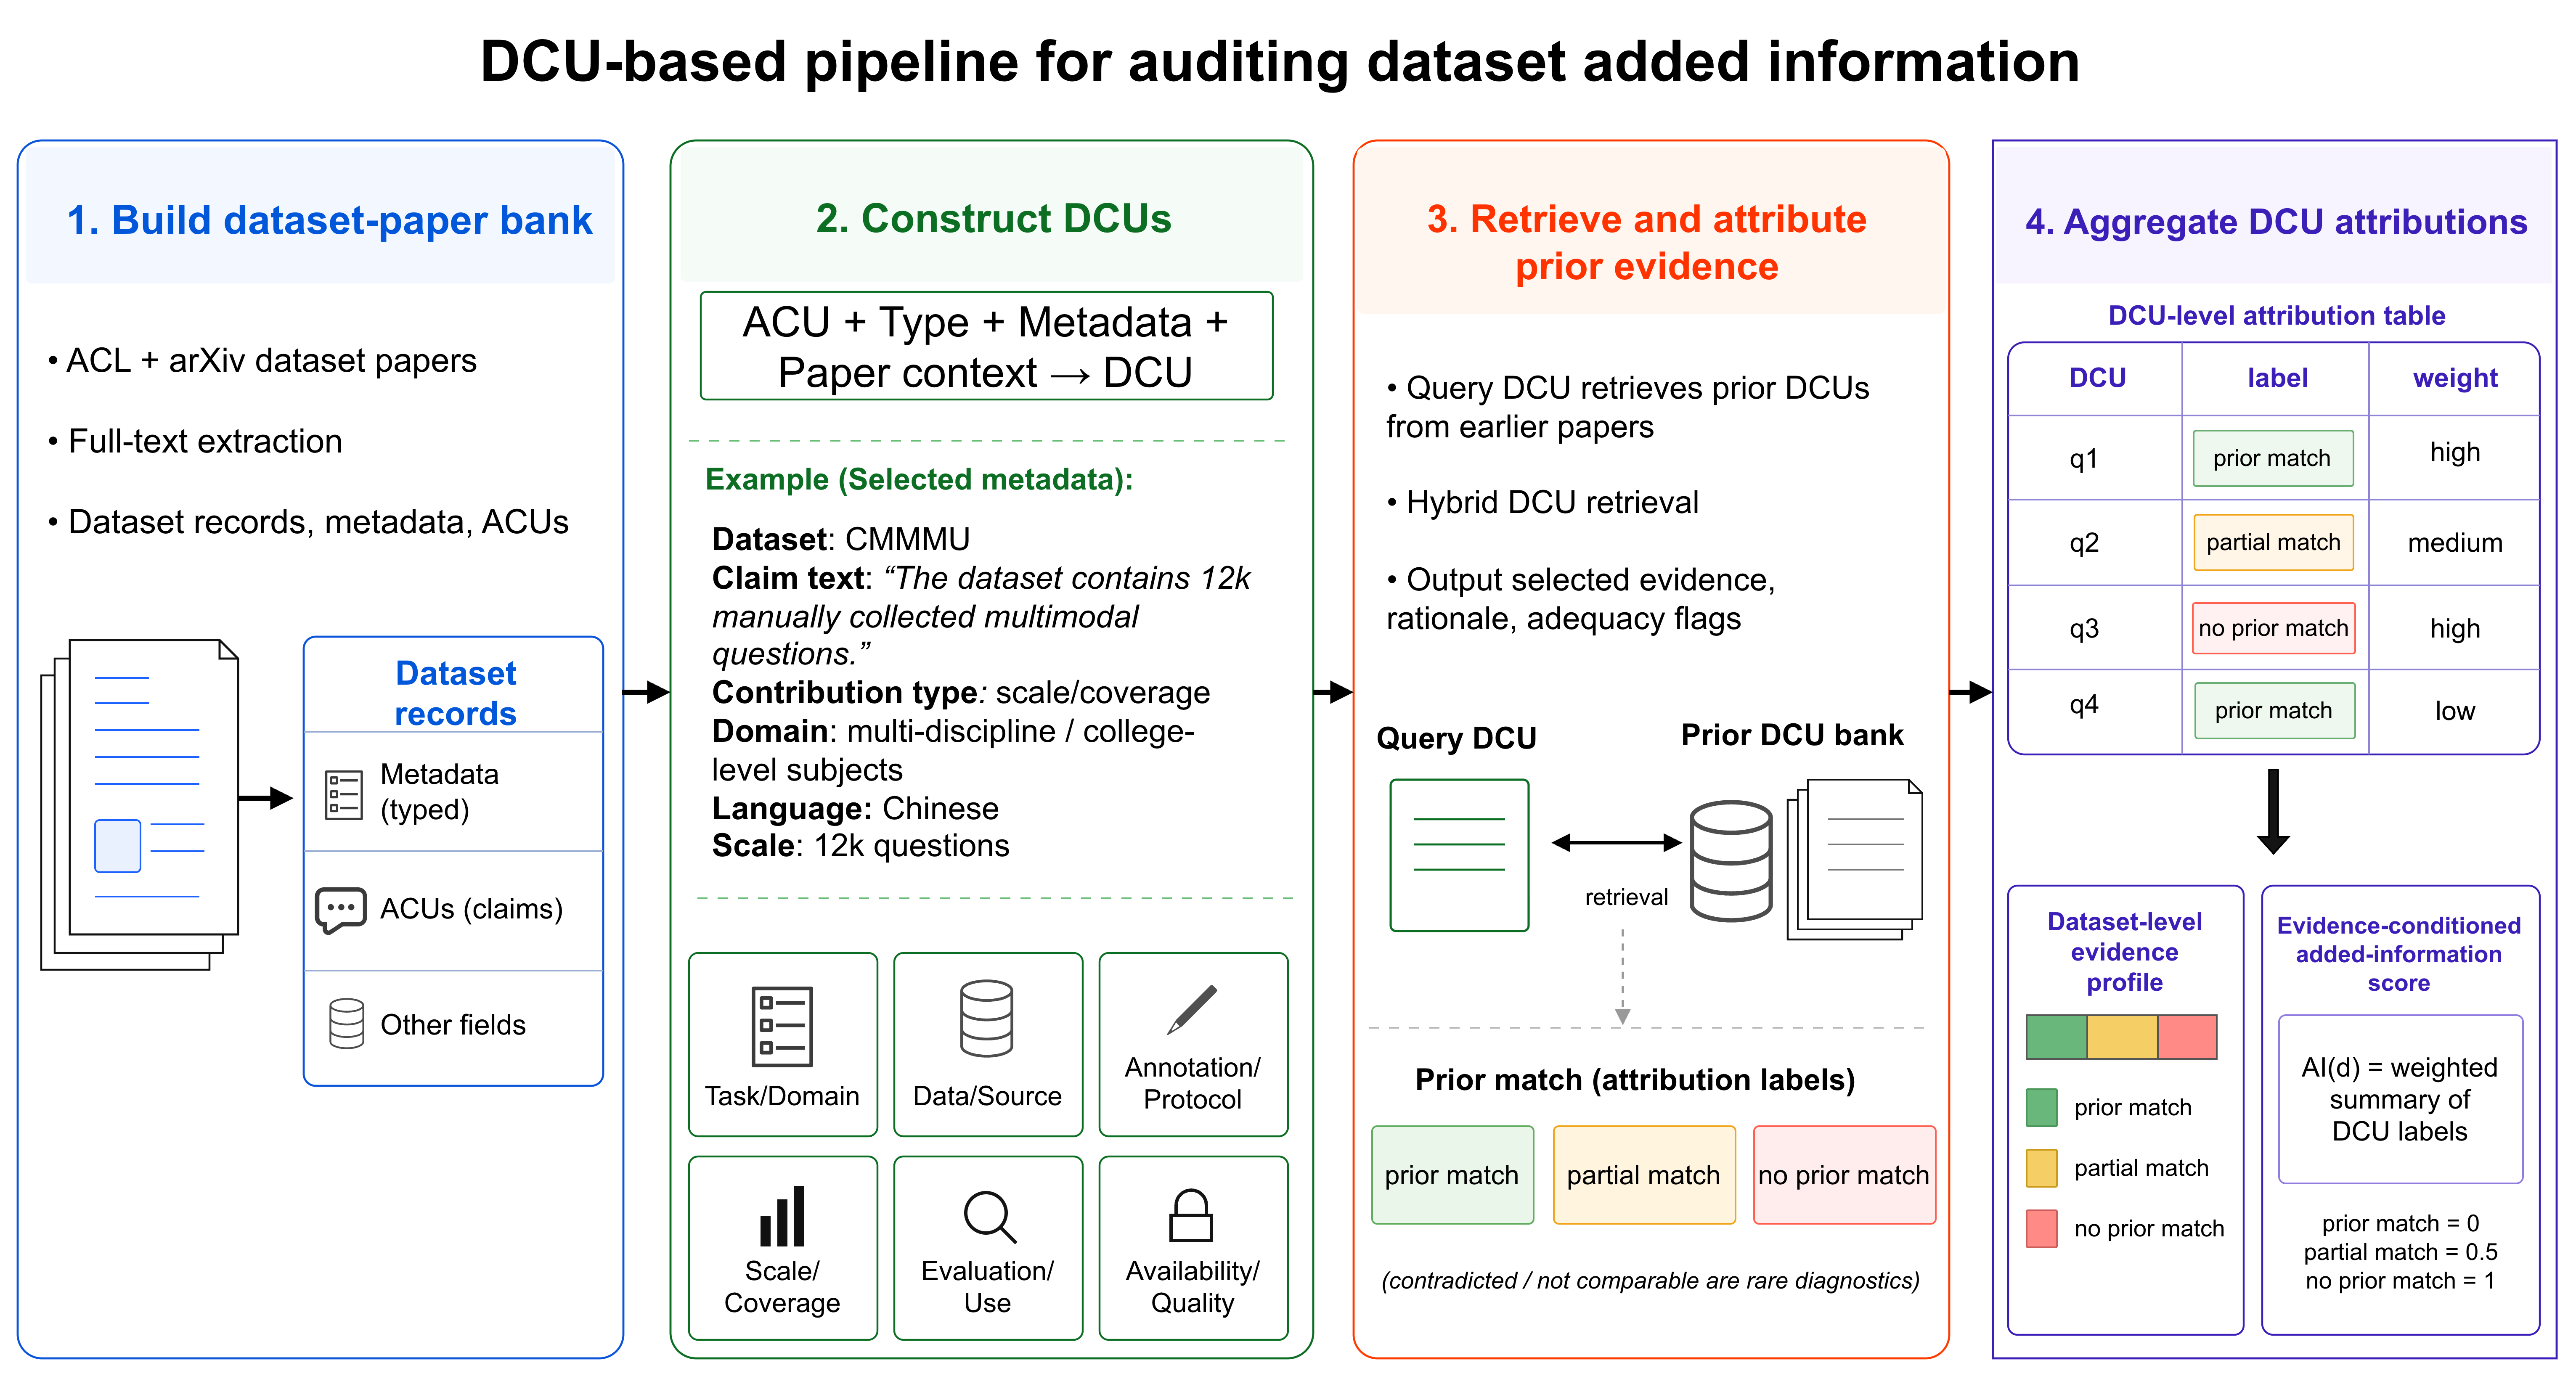
\includegraphics[width=0.72\linewidth]{figures/figure1_pipeline_overview.png}
\caption{Overview of the DCU-based pipeline for auditing dataset added information.}
\label{fig:pipeline}
\end{figure*}
Our goal is not to produce a global novelty leaderboard for datasets, nor only to improve scientific-document retrieval.
Instead, we use retrieval as one component of a broader framework for answering a practical question faced by dataset authors, reviewers, and users: \emph{what does this dataset add relative to prior datasets?}
Our contributions are:

\begin{enumerate}
    \item \textbf{A framework for evidence-conditioned dataset contribution analysis.} We define added information as a relation between dataset contribution claims and prior dataset evidence, and introduce DCUs as the unit for making this relation auditable.
    \item \textbf{A validated DCU-level retrieval and attribution pipeline.} We build a benchmark showing that structured DCU retrieval recovers prior evidence more effectively than paper-level or claim-text baselines, and validate extraction and attribution with human audits.
    \item \textbf{A corpus-scale analysis of recent NLP dataset papers.} Applying the framework to a 2023--2025 ACL/arXiv corpus shows that recent datasets most often add information through scale and coverage, while LLM-assisted construction is rapidly growing but does not correspond to higher added-information scores.
\end{enumerate}



\section{Task Formulation and Dataset Contribution Units}
This section formalizes the object that our system retrieves and attributes.
We first define added information as an evidence-indexed relation between query dataset claims and prior dataset evidence.
We then define Dataset Contribution Units, the structured claim representation used throughout retrieval, attribution, and corpus-scale analysis.
\subsection{From Novelty Judgments to Evidence Matching}
In this work, added information means: what remains in a dataset contribution claim after accounting for retrieved prior dataset evidence.
Let $d$ be a dataset introduced or substantially modified in a paper, and let $Q(d) = \{q_1, \ldots, q_m\}$ be its query DCUs.
Let $\evidence_t$ be an evidence index containing prior DCUs available before the query paper's publication time $t$.
For each query DCU $q_i$, the system retrieves candidate prior DCUs $P_i \subset \evidence_t$ and assigns an evidence-match label:
\begin{equation}
    y_i \in \mathcal{Y}.
\end{equation}
We use five evidence-match labels: prior-evidence match, partial prior-evidence match, no prior-evidence match, contradicted, and not comparable.
A \emph{prior-evidence match} means that a retrieved prior DCU already expresses the same dataset contribution.
A \emph{partial prior-evidence match} means that the prior DCU overlaps with the query claim but differs along an important dimension, such as domain, language, source, annotation protocol, scale, or release setting.
A \emph{no prior-evidence match} label means that none of the retrieved prior DCUs matches or partially matches the query claim.

The dataset-level output is the distribution of these labels, together with selected prior evidence and adequacy diagnostics:
\begin{equation}
    \ai_{\evidence_t}(d) = \operatorname{Aggregate}\big(\{(q_i, y_i, P_i, w_i)\}_{i=1}^m\big).
\end{equation}
We use the subscript $\evidence_t$ to emphasize that added information is conditional on the evidence index.
Thus, our framework produces an evidence-qualified contribution profile rather than an absolute novelty judgment.
Because retrieved evidence may be incomplete, every attribution is interpreted under an explicit evidence index; Section~\ref{sec:evidence_adequacy} defines how we filter corpus-level analyses when evidence is insufficient.
\subsection{Dataset Contribution Units}
We first extract atomic contribution claims from each dataset paper, building on prior work that decomposes generated text into atomic facts or atomic content units for fine-grained evidence checking \citep{min2023factscore,wan2024acueval}.
A \emph{Dataset Contribution Unit} (DCU) represents one such claim together with the dataset and paper information needed to compare it against prior work:
\begin{equation}
    \dcu = (c,\tau,m_d,p_d),
\end{equation}
where $c$ is the claim text, $\tau$ is the contribution type, $m_d$ is dataset metadata, and $p_d$ is paper context.

Dataset metadata includes fields such as the dataset name, task, domain, language, modality, data source, construction method, annotation protocol, scale, release status, and access conditions.
Paper context includes the paper title, year, venue, and the evidence span from which the claim was extracted.
We use six contribution types: task and domain, data source, annotation protocol, scale and coverage, evaluation use, and availability and quality.
\section{Dataset-Paper Corpus and Attribution Pipeline}
\label{sec:pipeline}

This section describes the corpus and pipeline used for corpus-scale added-information analysis.
We first construct an integrated corpus of recent NLP dataset papers and extract dataset metadata and DCUs from full text.
We then retrieve earlier DCUs as candidate prior evidence, attribute each query DCU against this evidence, and aggregate DCU-level labels into dataset-level contribution profiles.
Section~\ref{sec:retrieval_benchmark} evaluates the central retrieval subproblem; the present section describes how the full pipeline is run at scale.
\subsection{Corpus Construction}
We construct a corpus of recent NLP dataset papers from ACL Anthology and an NLP-oriented arXiv pool between 2023 and 2025.
The arXiv pool includes cs.CL papers and papers in adjacent categories that are identified as NLP-relevant by metadata and abstract screening.
The corpus supports two roles: recent papers provide query datasets for corpus-scale analysis, and earlier papers provide prior DCUs for the evidence index. 
\subsection{Dataset-Paper Identification}
We screen papers for whether they introduce, substantially modify, or release a dataset or benchmark.
The screen uses an abstract-level dataset-introduction classifier, followed by full-text extraction for positive papers.
We validate the screening classifier against two human annotators on a held-out corpus sample, obtaining 0.983--0.993 accuracy; details of the validation protocol and confusion matrices appear in Appendix~\ref{app:classifier_validation}.
\subsection{Metadata and DCU Extraction}

For each dataset-introducing paper, we extract dataset records, dataset-scoped metadata, and atomic contribution claims.
The metadata fields cover the dimensions needed for evidence comparison, including task, domain, language, source, construction method, annotation protocol, scale, release status, and access conditions.
These fields are informed by dataset documentation and data-lifecycle work \citep{gebru2021datasheets,bender2018data,pushkarna2022data,paullada2021data,holland2018nutrition}; prompt summaries and schema details appear in Appendix~\ref{app:llm_usage}.
Atomic contribution claims become DCUs after adding contribution type, dataset metadata, and paper context.
The resulting corpus contains 22,133 papers, 22,874 dataset records, and 77,571 DCUs across 2023--2025; Appendix~\ref{app:corpus_stats} reports the ACL/arXiv and year breakdown.
The integrated corpus grows from 4,820 extracted dataset records in 2023 to 10,441 in 2025, motivating scalable tools for organizing and comparing dataset contributions.
\subsection{Corpus-Scale Prior-Evidence Retrieval and Attribution}
\label{sec:corpus_attribution}

The corpus-scale pipeline applies the DCU representation to every extracted dataset record.
For each query DCU, we retrieve the top-50 prior DCUs from papers published before the query paper, using the Hybrid DCU retriever evaluated in Section~\ref{sec:retrieval_benchmark}.
For each dataset record, we then merge the retrieved candidates across all query DCUs into a compact deduplicated evidence set and ask the attribution model to label all query DCUs in a single structured prompt.
Dataset-level prompting avoids repeatedly presenting the same prior evidence for different claims from the same dataset and allows attribution decisions to share dataset context.
This follows the broader strategy of decomposing global judgments into atomic evidence checks rather than asking for a single undifferentiated score \citep{min2023factscore,wan2024acueval}.

Concretely, the pipeline retrieves the top-50 prior DCUs for each query DCU, merges them into a deduplicated dataset-level evidence set, and outputs evidence-match labels, selected evidence, rationales, adequacy judgments, and missing-prior-risk flags.
The attribution model outputs structured JSON containing, for each query DCU, its evidence-match label, selected prior evidence, importance weight, rationale, and adequacy diagnostics.
Across the completed 2024--2025 corpus-scale run, the pipeline produces 61,204 query-DCU attributions over 18,053 successfully processed dataset records.
Appendix~\ref{app:llm_usage} reports the LLM backends, decoding settings, and prompt summaries used for screening, extraction, attribution, and hosted-description alignment.
Appendix~\ref{app:worked_example} shows a concrete CMedCalc-Bench example in which different DCUs from the same dataset receive different prior-evidence attributions.
\subsection{Evidence Adequacy Filtering}
\label{sec:evidence_adequacy}

Because the evidence index may be incomplete, the attribution model also records whether the retrieved prior evidence is sufficient to interpret each DCU-level label and whether the case has high missing-prior risk.
For corpus-scale added-information analyses, we retain only dataset records that pass a record-level evidence-adequacy filter over these diagnostics.
This filter is intended to prevent no-prior-match labels from being interpreted when retrieved evidence is too sparse or mismatched; the diagnostic definitions and thresholds are provided in Appendix~\ref{app:evidence_adequacy_details}.
\subsection{From Claim Labels to Dataset Profiles}
\label{sec:dataset_profiles}

After attribution, we summarize each dataset record by its DCU-level evidence profile: the proportion of DCUs with prior matches, partial matches, no prior matches, contradictions, or not-comparable judgments; the no-prior-match rate by DCU type; and evidence adequacy diagnostics.
For corpus-scale analysis, we also compute an evidence-conditioned added-information score:
\begin{equation}
    \mathrm{AI}(d) =
    \frac{\sum_i w_i s(y_i)}{\sum_i w_i},
\end{equation}
where $y_i$ is the evidence-match label for query DCU $i$, $w_i$ is the claim-importance weight, and $s(y_i)$ maps prior match to $0$, partial prior match to $0.5$, and no prior match to $1$.

This ordinal mapping assigns no added-information mass to already matched claims, maximum mass to claims with no retrieved prior match, and an intermediate value to claims that overlap prior evidence but differ along a contribution dimension; Appendix~\ref{app:score_mapping} discusses the mapping.
Contradicted and not-comparable labels are excluded from the score and reported separately.
The score is therefore a compact summary of the DCU-level evidence profile, not an absolute novelty label.
\paragraph{Validation summary.}
Before applying the pipeline at corpus scale, we validate DCU construction and attribution through human audit, and we separately check whether paper-derived dataset descriptions align with hosted dataset evidence.
The human audit shows high reliability for DCU construction (98.6\% claim groundedness and 99.3\% type accuracy), selected prior evidence (92.9\% precision), and attribution rationales (98.7\% groundedness).
Agreement with model-assigned evidence-match labels is lower, at 76.3--77.4\% of audited cases, reflecting that the final match label is the most judgment-sensitive step rather than a fully automatic ground truth.
The disagreements are mainly boundary cases in whether retrieved evidence should count as a direct prior match, a partial match, or no prior match, rather than failures to ground the DCU or rationale.
As a separate consistency check, we compare paper-derived descriptions for 79 released datasets against independently available dataset cards, README files, metadata, and sample rows.
Appendix~\ref{app:validation_details} reports the audit protocol, agreement breakdown, hosted-source validation, and metric definitions.
\section{DCU-Level Prior Evidence Retrieval Benchmark}
\label{sec:retrieval_benchmark}

The full pipeline depends on retrieving prior evidence at the same granularity at which added information is defined.
We therefore evaluate the central retrieval subproblem: whether systems can recover human-confirmed prior DCUs for a query DCU from the full prior-DCU evidence index.
This benchmark tests whether prior-evidence retrieval should operate over papers, atomic claim text, or structured Dataset Contribution Units.
We compare first-stage retrievers based on BM25, dense embedding retrieval, and their hybrid combination.
Unlike dataset search systems that retrieve dataset pages or metadata records for a user query \citep{noy2019google,chapman2020dataset,viswanathan2023datafinder}, our task retrieves prior evidence units for a specific dataset contribution claim.
The experiment isolates two design choices: the unit being scored and the representation used for scoring.
\subsection{Benchmark Construction}
We build a manually curated benchmark from 100 sampled dataset papers.
For each query dataset, annotators identify prior dataset or benchmark papers discussed by the authors.
They then inspect the DCUs extracted from these cited prior papers and label which prior DCUs match or partially match each query DCU.

The validated benchmark contains 160 query DCUs with at least one gold prior DCU and 311 gold prior-DCU pairs. 
We treat this benchmark as a targeted diagnostic for comparing retrieval representations, not as training data or as the source of corpus-scale findings; its manually verified labels are costly because annotators must inspect cited prior papers at the DCU level.
At evaluation time, systems must retrieve these gold prior DCUs from the full prior-DCU evidence index, rather than from the cited papers alone.
This design uses cited papers to create high-precision evidence labels while still evaluating global prior-evidence retrieval.
\subsection{Metrics}
We report three positive retrieval metrics in the main table.
Hit@$k$ measures whether at least one gold prior DCU appears in the top $k$ retrieved DCUs.
MRR measures how early the first gold prior DCU is ranked.
nDCG@$10$ uses graded gains, assigning higher gain to direct prior-evidence matches than partial matches.
\subsection{Retrieval Methods}
All methods receive the same query DCU and rank candidate prior DCUs from the full prior-DCU evidence index.
They differ along three axes: whether they score papers or DCUs, how much structure is included in the representation, and whether lexical and dense scores are combined.
BM25 is a standard sparse lexical retrieval baseline \citep{robertson2009probabilistic}, while dense retrieval encodes query and candidate text with sentence or document embeddings \citep{reimers2019sentence}.
\paragraph{Paper-level baselines.}
These methods first rank prior papers and then assign each paper score to all DCUs extracted from that paper.
We test title+abstract, paper-level contribution summary, and full-text representations.
These baselines ask whether DCU-level retrieval is necessary, or whether finding the right prior paper is sufficient.
They are motivated by scientific document retrieval methods that learn paper representations for relatedness and recommendation \citep{cohan2020specter,ostendorff2022scincl}.
Full-text dense retrieval uses the encoder's maximum input window over extracted paper text; we include it as a diagnostic baseline and do not use it in the final pipeline.
\paragraph{Claim-text baselines.}
ACU text uses only the atomic claim text.
ACU type+text additionally prepends the contribution type.
For each representation, we evaluate BM25, dense, and hybrid retrieval.
These baselines test whether atomized claims alone contain enough information for prior evidence retrieval.
Atomic-unit retrieval has also been used to improve RAG chunk recall by decomposing chunks into atomic statements and synthetic questions \citep{raina2024question}.
\paragraph{DCU methods.}
BM25 DCU and Dense DCU serialize the full DCU and score it using lexical or dense retrieval.
Hybrid DCU combines BM25 and dense scores over the full DCU serialization, and is our default first-stage retriever for corpus-scale attribution.
Hybrid scores min--max normalize BM25 and dense scores within the candidate set and average them with equal weight.
\begin{table*}[t]
\centering
\scriptsize
\setlength{\tabcolsep}{3pt}
\begin{tabular}{lllrrrrr}
\toprule
Family & Representation & Scorer & Hit@1 & Hit@10 & Hit@50 & MRR & nDCG@10 \\
\midrule
\textit{Lower} & Random DCU & Random & 0.000 & 0.037 & 0.175 & 0.016 & 0.010 \\
\midrule
Paper & Contribution summary & Hybrid & 0.319 & 0.756 & 0.900 & 0.465 & 0.508 \\
Claim & ACU text & Hybrid & 0.219 & 0.487 & 0.669 & 0.308 & 0.263 \\
DCU & Full DCU & BM25 & \textbf{0.456} & 0.812 & 0.956 & 0.586 & 0.597 \\
DCU & Full DCU & Hybrid & 0.450 & \textbf{0.894} & \textbf{0.963} & \textbf{0.602} & \textbf{0.633} \\
\bottomrule
\end{tabular}
\caption{Representative DCU-level prior evidence retrieval results. The full retrieval table appears in Appendix~\ref{app:full_retrieval_results}.}
\label{tab:dcu_retrieval}
\end{table*}
Table~\ref{tab:dcu_retrieval} compares paper-level, claim-text, and structured DCU retrieval, testing whether DCU-level prior evidence requires dataset metadata and paper context.
The results support three conclusions.
First, paper-level retrieval is insufficient for DCU-level evidence ranking.
The best paper-level baseline, Paper Summary Hybrid, reaches 0.465 MRR and 0.756 Hit@10, while Hybrid DCU reaches 0.602 MRR and 0.894 Hit@10.
Ranking papers and expanding their scores to all contained DCUs therefore misses the fine-grained evidence needed for DCU-level attribution.

Second, atomization alone is not enough.
ACU-only and typed-ACU methods underperform paper-level baselines across positive retrieval metrics, indicating that short atomic claims lack enough context for retrieval even when BM25 and dense signals are combined.

Third, DCU structure matters.
BM25 DCU and Hybrid DCU achieve the strongest positive retrieval results, showing that fielded dataset context makes DCU-level evidence retrievable.
Hybrid DCU obtains the best Hit@10, Hit@50, MRR, and nDCG@10, while BM25 DCU is slightly better at Hit@1.
We therefore use Hybrid DCU retrieval as the first-stage retriever for corpus-scale attribution.
\section{Corpus-Scale Findings}

We now apply the pipeline to the integrated dataset-paper corpus.
Across the 2024--2025 run, 11,046 of 18,053 successfully processed dataset records pass the evidence-adequacy filters in Section~\ref{sec:evidence_adequacy}, yielding 37,776 scored query DCUs for analysis.
The resulting dataset-level added-information scores have mean 0.566 and median 0.500.
We use the corpus-scale analysis to ask two descriptive questions about recent NLP dataset papers.
First, what contribution dimensions do dataset papers emphasize, and where do they most often differ from retrieved prior dataset evidence?
Second, as LLM-assisted construction becomes more common, does it correspond to higher evidence-conditioned added information?
\subsection{Q1: What Contribution Dimensions Do Recent Dataset Papers Emphasize?}
\begin{figure*}[t]
\centering
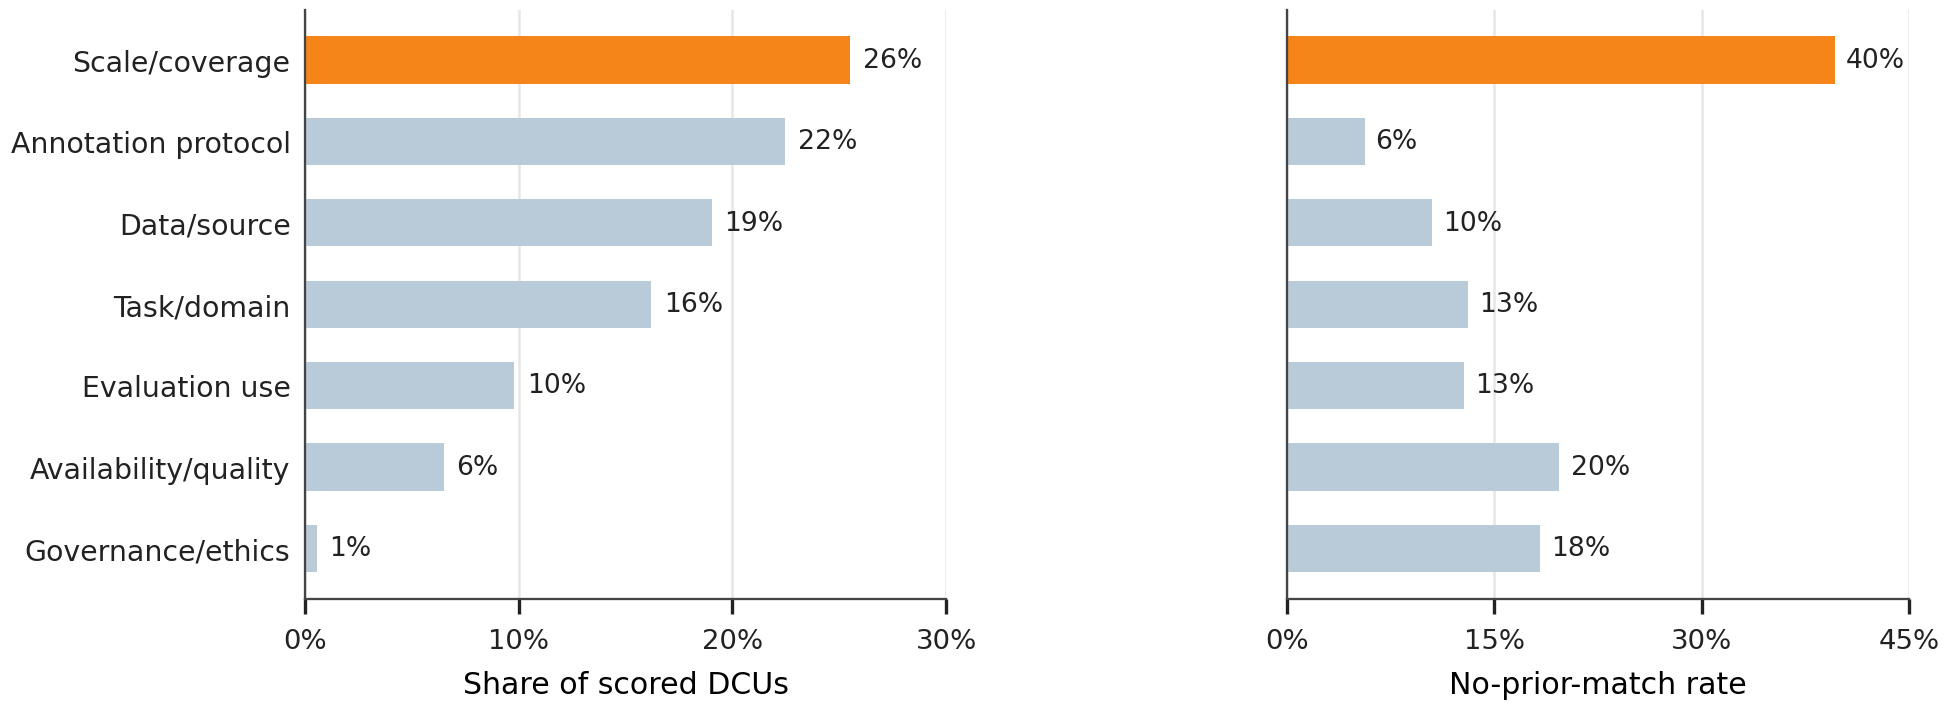
\includegraphics[width=0.76\linewidth]{figures/figure3_contribution_directions.png}
\caption{
Contribution dimensions in corpus-scale DCU attributions.
The left panel shows where scored DCUs concentrate; the right panel shows the share of DCUs in each dimension with no retrieved prior-evidence match.
}
\label{fig:contribution_directions}
\end{figure*}
To answer this question, we examine two DCU-level quantities.
The first is the share of scored DCUs assigned to each contribution type, which measures where dataset papers place their contribution claims.
The second is the no-prior-match rate within each type, which measures where claims most often lack retrieved prior evidence.
Figure~\ref{fig:contribution_directions} plots these two quantities by contribution type.
Scale and coverage is the largest DCU category, accounting for 26\% of scored DCUs, followed by annotation protocol (22\%), data/source (19\%), and task/domain (16\%).
Scale and coverage is also the dimension with the largest evidence gap: 40\% of its DCUs receive no prior-evidence match, compared with 13\% for task/domain claims and 10\% for data/source claims.
The score decomposition leads to the same conclusion: scale and coverage contributes the largest share of total added-information score mass (30.1\%) and has the highest weighted mean claim score (0.687).
Together, these patterns suggest that recent dataset papers add information mostly through size, breadth, language or domain coverage, evaluation coverage, and construction scope, rather than through entirely new tasks or sources.
By contrast, governance/ethics, availability/quality, and evaluation/use claims are much smaller parts of the scored DCU profile.
Appendix~\ref{app:corpus_diagnostics} reports supporting task and domain landscapes, including the most common tasks and domains in the corpus.
\subsection{Q2: Does LLM-Assisted Construction Lead to More Added Information?}
\begin{figure*}[t]
\centering
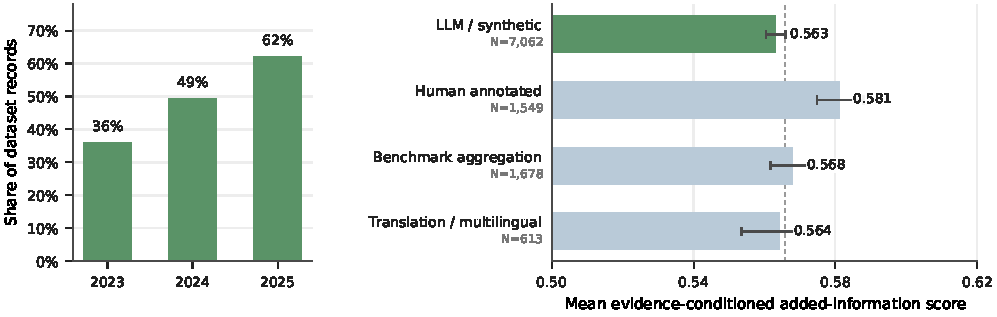
\includegraphics[width=0.70\linewidth]{figures/figure4_llm_score.pdf}
\caption{
The left panel shows the share of extracted dataset records whose construction uses an LLM.
The right panel shows mean added-information score by construction method, with bootstrap 95\% confidence intervals.
}
\label{fig:llm_score}
\end{figure*}
This question has two parts: whether LLM use is becoming more common in dataset construction, and whether LLM-assisted datasets add more information relative to prior evidence.
We measure the first by the share of extracted dataset records whose construction uses an LLM, and the second using the dataset-level score from Section~\ref{sec:dataset_profiles}.
Figure~\ref{fig:llm_score} shows both quantities.
LLM-assisted construction becomes increasingly common, rising from 36.0\% of extracted dataset records in 2023 to 49.4\% in 2024 and 62.1\% in 2025.
However, this construction shift does not correspond to higher evidence-conditioned added-information scores.
LLM/synthetic records have a mean score of 0.563, compared with 0.568 for benchmark aggregation and 0.581 for human-annotated records.
Thus, LLMs are changing how NLP datasets are produced, but not necessarily what they add relative to retrieved prior dataset evidence.
LLM-assisted datasets appear to be rapidly expanding within existing task, source, and evaluation frames, rather than systematically producing claims with less prior evidence.
\paragraph{Additional diagnostics.}
We also analyze prior-dataset relationship types, primary use, resource type, language and scale groups, task/domain clusters, documentation and governance features, institution sector, and year/source profiles.
These analyses are reported in Appendix~\ref{app:corpus_diagnostics}.
They support the same overall interpretation: dataset papers are usually anchored in prior tasks, sources, or evaluation settings, while the clearest evidence gaps appear in scale, coverage, breadth, and construction scope.
\section{Related Work}
Prior work on dataset and benchmark measurement argues that dataset properties require explicit construct definitions and validation before scores can support scientific claims \citep{bean2025construct,raji2021benchmark,zhao2024measure,jacobs2021measurement}.
This concern is especially relevant for dataset novelty, which is often invoked as an intuitive paper-level property but depends on the contribution dimension being compared.
Unlike metrics for model difficulty, usable information, diversity, hardness, or separability \citep{ethayarajh2022understanding,mitchell2022measuring,vivek2024anchor,friedman2023vendi,yao2025measure}, we define added information as an evidence-indexed relation between typed dataset claims and prior dataset evidence.

Dataset documentation and data-lifecycle work identify fields needed for interpretation and reuse, including motivation, composition, provenance, access conditions, and governance \citep{gebru2021datasheets,bender2018data,pushkarna2022data,holland2018nutrition,paullada2021data}.
These fields are not only reporting desiderata: they determine whether two dataset claims concern the same task, source, annotation process, scale, release condition, or use case.
Our schema draws on these dimensions, but uses extracted metadata to contextualize contribution claims rather than proposing another documentation template.

Our DCU representation also builds on fine-grained evidence evaluation.
Summarization evaluation, factuality, consistency, fact verification, and RAG work decompose documents or generated text into smaller content units and verify each unit against evidence \citep{nenkova2004pyramid,min2023factscore,wan2024acueval,fabbri2022qafacteval,laban2022summac,thorne2018fever,raina2024question}.
DCUs adapt this unit-based view to dataset contributions, where claims about benchmarks, sources, annotation protocols, scale, or release conditions often require dataset metadata and paper context.
Information retrieval work provides lexical, dense, and scientific-document baselines for ranking papers, passages, or datasets \citep{robertson2009probabilistic,reimers2019sentence,cohan2020specter,ostendorff2022scincl,noy2019google,chapman2020dataset,viswanathan2023datafinder}.
Our retrieval target is more specific: for each query DCU, the system must recover earlier DCUs that match or partially match the same contribution dimension, since a topically related paper may not provide evidence for a particular claim.

Finally, our corpus-scale analysis uses LLM-assisted screening, extraction, and attribution, making it closer to technology-assisted evidence synthesis than to fully automatic measurement.
Prior work on systematic-review automation emphasizes that machine assistance can reduce screening and extraction effort, but requires explicit protocols, validation, and human oversight \citep{marshall2019automation,thomas2011textmining,wang2024zeroshot}.
Following this principle, we separate extraction, retrieval, attribution, evidence adequacy, and human audit, and report validation rather than treating LLM outputs as definitive measurements \citep{bean2025construct,artstein2008intercoder}.
\section{Conclusion}
We introduced a dataset-contribution framework for auditing added information in NLP dataset papers.
By representing dataset contributions as DCUs, retrieving prior DCUs, and attributing evidence matches under adequacy constraints, the framework reframes dataset novelty as an auditable relation between claims and prior evidence.
Applied to recent ACL/arXiv dataset papers, it supports a large-scale analysis of how NLP datasets are constructed, reused, released, governed, and differentiated from prior work.
The central output is not a global novelty ranking, but an evidence-conditioned map of dataset contribution claims and their relation to prior evidence. 
Such a map can support the decisions that motivate the task: helping authors position a new dataset, helping reviewers assess overlap with prior work, and helping dataset users identify which contribution dimensions may justify adoption.
\section{Limitations}

\smallskip\noindent\textbf{Evidence index incompleteness.}\par\noindent
Our added-information estimates are conditional on the evidence index.
Relevant prior datasets may appear outside ACL/arXiv, in older papers, non-NLP venues, dataset cards, technical reports, or project pages.
We mitigate this with evidence adequacy filters, but cannot claim global novelty.

\smallskip\noindent\textbf{Citation-grounded benchmark bias.}\par\noindent
The benchmark uses cited prior papers to construct labels.
Citations provide a high-precision source of prior evidence but may omit relevant uncited prior work.

\smallskip\noindent\textbf{LLM extraction and attribution errors.}\par\noindent
Although we validate attribution against human auditors, errors remain possible, especially for subtle partial-match distinctions, missing-prior-risk judgments, and noisy metadata extraction.

\smallskip\noindent\textbf{Descriptive rather than causal analysis.}\par\noindent
Corpus-scale findings are descriptive associations.
We do not claim that specific construction practices cause higher adoption, reuse, or added information.

\smallskip\noindent\textbf{Temporal scope.}\par\noindent
We focus on 2023--2025 ACL/arXiv papers and use earlier-year prior DCUs for attribution.
This design supports recent ecosystem analysis but does not cover the full history of NLP datasets.
\section{Ethical Considerations}
This work analyzes publicly available research papers and metadata.
The main ethical risk is overinterpretation: readers may treat a no-prior-match claim as proof of novelty or a low added-information profile as evidence that a dataset is unimportant.
This risk parallels broader concerns that dataset and benchmark scores can be overinterpreted when the construct and operationalization are not explicit \citep{raji2021benchmark,zhao2024measure,bean2025construct}.
We explicitly define all outputs as evidence-conditional and provide adequacy filters to prevent no-prior-match-under-index judgments from being treated as globally novel.
We will release prompts, annotation guidelines, and validation results to support reproducibility and critical inspection.
\bibliography{custom}
\clearpage
\appendix
\section{Appendix: Dataset-Paper Corpus Statistics}
\label{app:corpus_stats}

Table~\ref{tab:corpus_stats} reports the ACL/arXiv and year breakdown for the integrated dataset-paper corpus used by the retrieval and corpus-scale analyses.
\begin{table*}[h]
\centering
\small
\begin{tabular}{lrrrrrr}
\toprule
Corpus & Papers & Dataset records & DCUs & 2023 records & 2024 records & 2025 records \\
\midrule
ACL Anthology & 10,079 & 10,422 & 36,726 & 2,193 & 3,792 & 4,437 \\
arXiv NLP-oriented & 12,054 & 12,452 & 40,845 & 2,627 & 3,821 & 6,004 \\
Integrated & 22,133 & 22,874 & 77,571 & 4,820 & 7,613 & 10,441 \\
\bottomrule
\end{tabular}
\caption{Integrated 2023--2025 NLP dataset-paper corpus.}
\label{tab:corpus_stats}
\end{table*}

\subsection{Extended 2020--2025 Corpus Expansion and Metadata Enrichment}
\label{app:extended_corpus}

In addition to the 2023--2025 corpus used for the main DCU attribution analysis, we implemented an expanded 2020--2025 paper-catalog pipeline for downstream replication and extension.
The expanded ACL catalog contains 58,026 papers.
The repaired arXiv catalog contains 205,732 papers after targeted repair and deduplication by arXiv base identifier.
After removing duplicate arXiv titles and 16,983 ACL-title overlaps, the 2020--2025 arXiv screening set contains 188,687 papers.
Table~\ref{tab:extended_corpus_status} summarizes the current expansion artifacts.

\begin{table*}[h]
\centering
\small
\begin{tabular}{lrrl}
\toprule
Artifact & Rows / papers & Removed overlap & Status \\
\midrule
ACL 2020--2025 paper catalog & 58,026 & -- & complete at paper-catalog level \\
arXiv 2020--2025 repaired catalog & 205,732 & -- & repaired v2 catalog \\
arXiv 2020--2025 screening set & 188,687 & 16,983 ACL-title overlaps & ready for abstract screening \\
arXiv paper metadata enrichment & 188,687 & 99.48\% matched & complete \\
\bottomrule
\end{tabular}
\caption{Extended 2020--2025 corpus expansion status.}
\label{tab:extended_corpus_status}
\end{table*}

We ran a 1,000-paper abstract-screening pilot on the expanded arXiv screening set to validate the expanded classification path before scaling.
After deduplicating one repeated output row, the pilot contains 1,000 unique 2020 arXiv papers.
The classifier marked 328 papers as NLP-relevant, 520 as mentioning datasets, and 100 as dataset-introducing.
This pilot is used as a smoke test and cost-calibration sample; it is not treated as an estimate of the final 2020--2025 corpus rate.
We then ran a larger year-stratified 3,000-paper pilot with 500 arXiv screening records sampled from each year from 2020 through 2025.
After retrying and reconciling missing records from one failed batch, the clean pilot contains 3,000 unique papers with no missing paper IDs.
The classifier marked 1,077 papers as NLP-relevant, 1,758 as mentioning datasets, and 376 as dataset-introducing.
The dataset-introducing counts by year were 45, 57, 69, 60, 62, and 83 for 2020 through 2025, respectively.

We also added a public paper-metadata enrichment layer for the expanded arXiv catalog.
Using exact arXiv or DOI identifiers, Semantic Scholar metadata enrichment was completed for all 188,687 papers in the expanded arXiv screening set.
It matched 187,712 papers and recovered citation counts for the same 187,712 papers, corresponding to 99.48\% coverage; 975 papers remained unmatched.
Among matched papers, the median citation count was 6, the mean was 28.67, and the 90th percentile was 49.
Citation counts are interpreted as a point-in-time measure queried in August 2026, rather than a direct comparison of paper quality across publication years.
We also added a resource-level enrichment path for dataset-bank records with explicit hosted-resource URLs.
On the 2023--2025 integrated dataset bank, this path found 201 records with Hugging Face dataset links and recovered download counts for 212 of 218 Hugging Face dataset links (97.2\% link-level coverage).
A separate 50-record GitHub pilot recovered star/fork metadata for 46 of 50 GitHub links (92.0\% link-level coverage).
These metadata fields are point-in-time measurements and are stored with enrichment provenance, query timestamps, and exact URL or identifier match policies.

\section{Appendix: LLM Usage and Prompt Templates}
\label{app:llm_usage}

Table~\ref{tab:llm_usage} summarizes the LLM calls used in the pipeline.
All corpus-scale calls use structured prompts and JSON parsing.
For readability, we summarize the prompts in this appendix and place the verbatim prompt templates and JSON schemas in the replication package.
\begin{table*}[h]
\centering
\scriptsize
\setlength{\tabcolsep}{4pt}
\begin{tabular}{p{.24\linewidth}p{.24\linewidth}p{.22\linewidth}p{.20\linewidth}}
\toprule
Pipeline step & Model / backend & Decoding & Output used in paper \\
\midrule
Dataset-paper screening & \texttt{gpt-5.4-mini} / OpenAI Responses API & deterministic JSON prompt & dataset-introduction screen \\
Full-text metadata and DCU extraction & \texttt{gemini-3.1-flash-lite} / Gemini API & temperature 0; JSON output & dataset records, metadata fields, ACUs/DCUs \\
Corpus-scale attribution & \texttt{gemini-3.1-flash-lite} / Gemini API & temperature 0; JSON output & evidence-match labels, rationales, adequacy diagnostics, scores \\
Hosted-description alignment & LLM-assisted synthetic description generation & deterministic prompt; hosted evidence only & description-alignment consistency check \\
\bottomrule
\end{tabular}
\caption{LLM applications in the pipeline.}
\label{tab:llm_usage}
\end{table*}

\paragraph{Prompt summaries.}
The screening prompt presents paper title, abstract, venue/source metadata, and asks the model to decide whether the paper introduces, substantially modifies, or releases a dataset or benchmark.
The JSON output contains a binary dataset-paper decision, short rationale, and uncertainty flags.
The instruction explicitly excludes papers that only use existing datasets for model training or evaluation without introducing a new or substantially modified resource.
The full-text extraction prompt presents the paper text and asks for a list of dataset records.
For each record, the model outputs dataset identity, role, resource type, intended use, task, domain, language, modality, source data, construction method, annotation protocol, scale, release/access fields, governance fields, and atomic contribution claims.
Each ACU must include claim text, contribution type, importance, evidence span, and paper section.
The parser normalizes these fields into DCUs by combining claim text, contribution type, dataset metadata, and paper context.
The attribution prompt presents all query DCUs for one dataset record together with a deduplicated set of retrieved prior DCUs from earlier papers.
For each query DCU, the model must select one of five labels: prior-evidence match, partial prior-evidence match, no prior-evidence match, contradicted, or not comparable.
It must also return selected prior DCU ids, a short evidence-grounded rationale, an evidence-adequacy judgment, a missing-prior-risk flag, and an importance label.
The prompt instructs the model to use no-prior-match only when the displayed prior evidence does not match or partially match the query claim, and to flag high missing-prior risk when retrieved evidence is too sparse, generic, or mismatched for interpretation.
Human auditors see the query DCU, its dataset context, retrieved prior evidence, the model-assigned label, selected evidence, and rationale.
They judge whether the claim is grounded, whether the DCU type is correct, whether selected evidence is useful, whether the rationale is grounded, and whether they accept the final evidence-match label.
For label audits, auditors may either accept the model label or provide a corrected label from the same five-label inventory.

\section{Appendix: Worked Attribution Example}
\label{app:worked_example}

Figure~\ref{fig:worked_example} shows a CMedCalc-Bench example in which different DCUs from the same dataset receive different prior-evidence attributions.
\begin{figure*}[h]
\centering
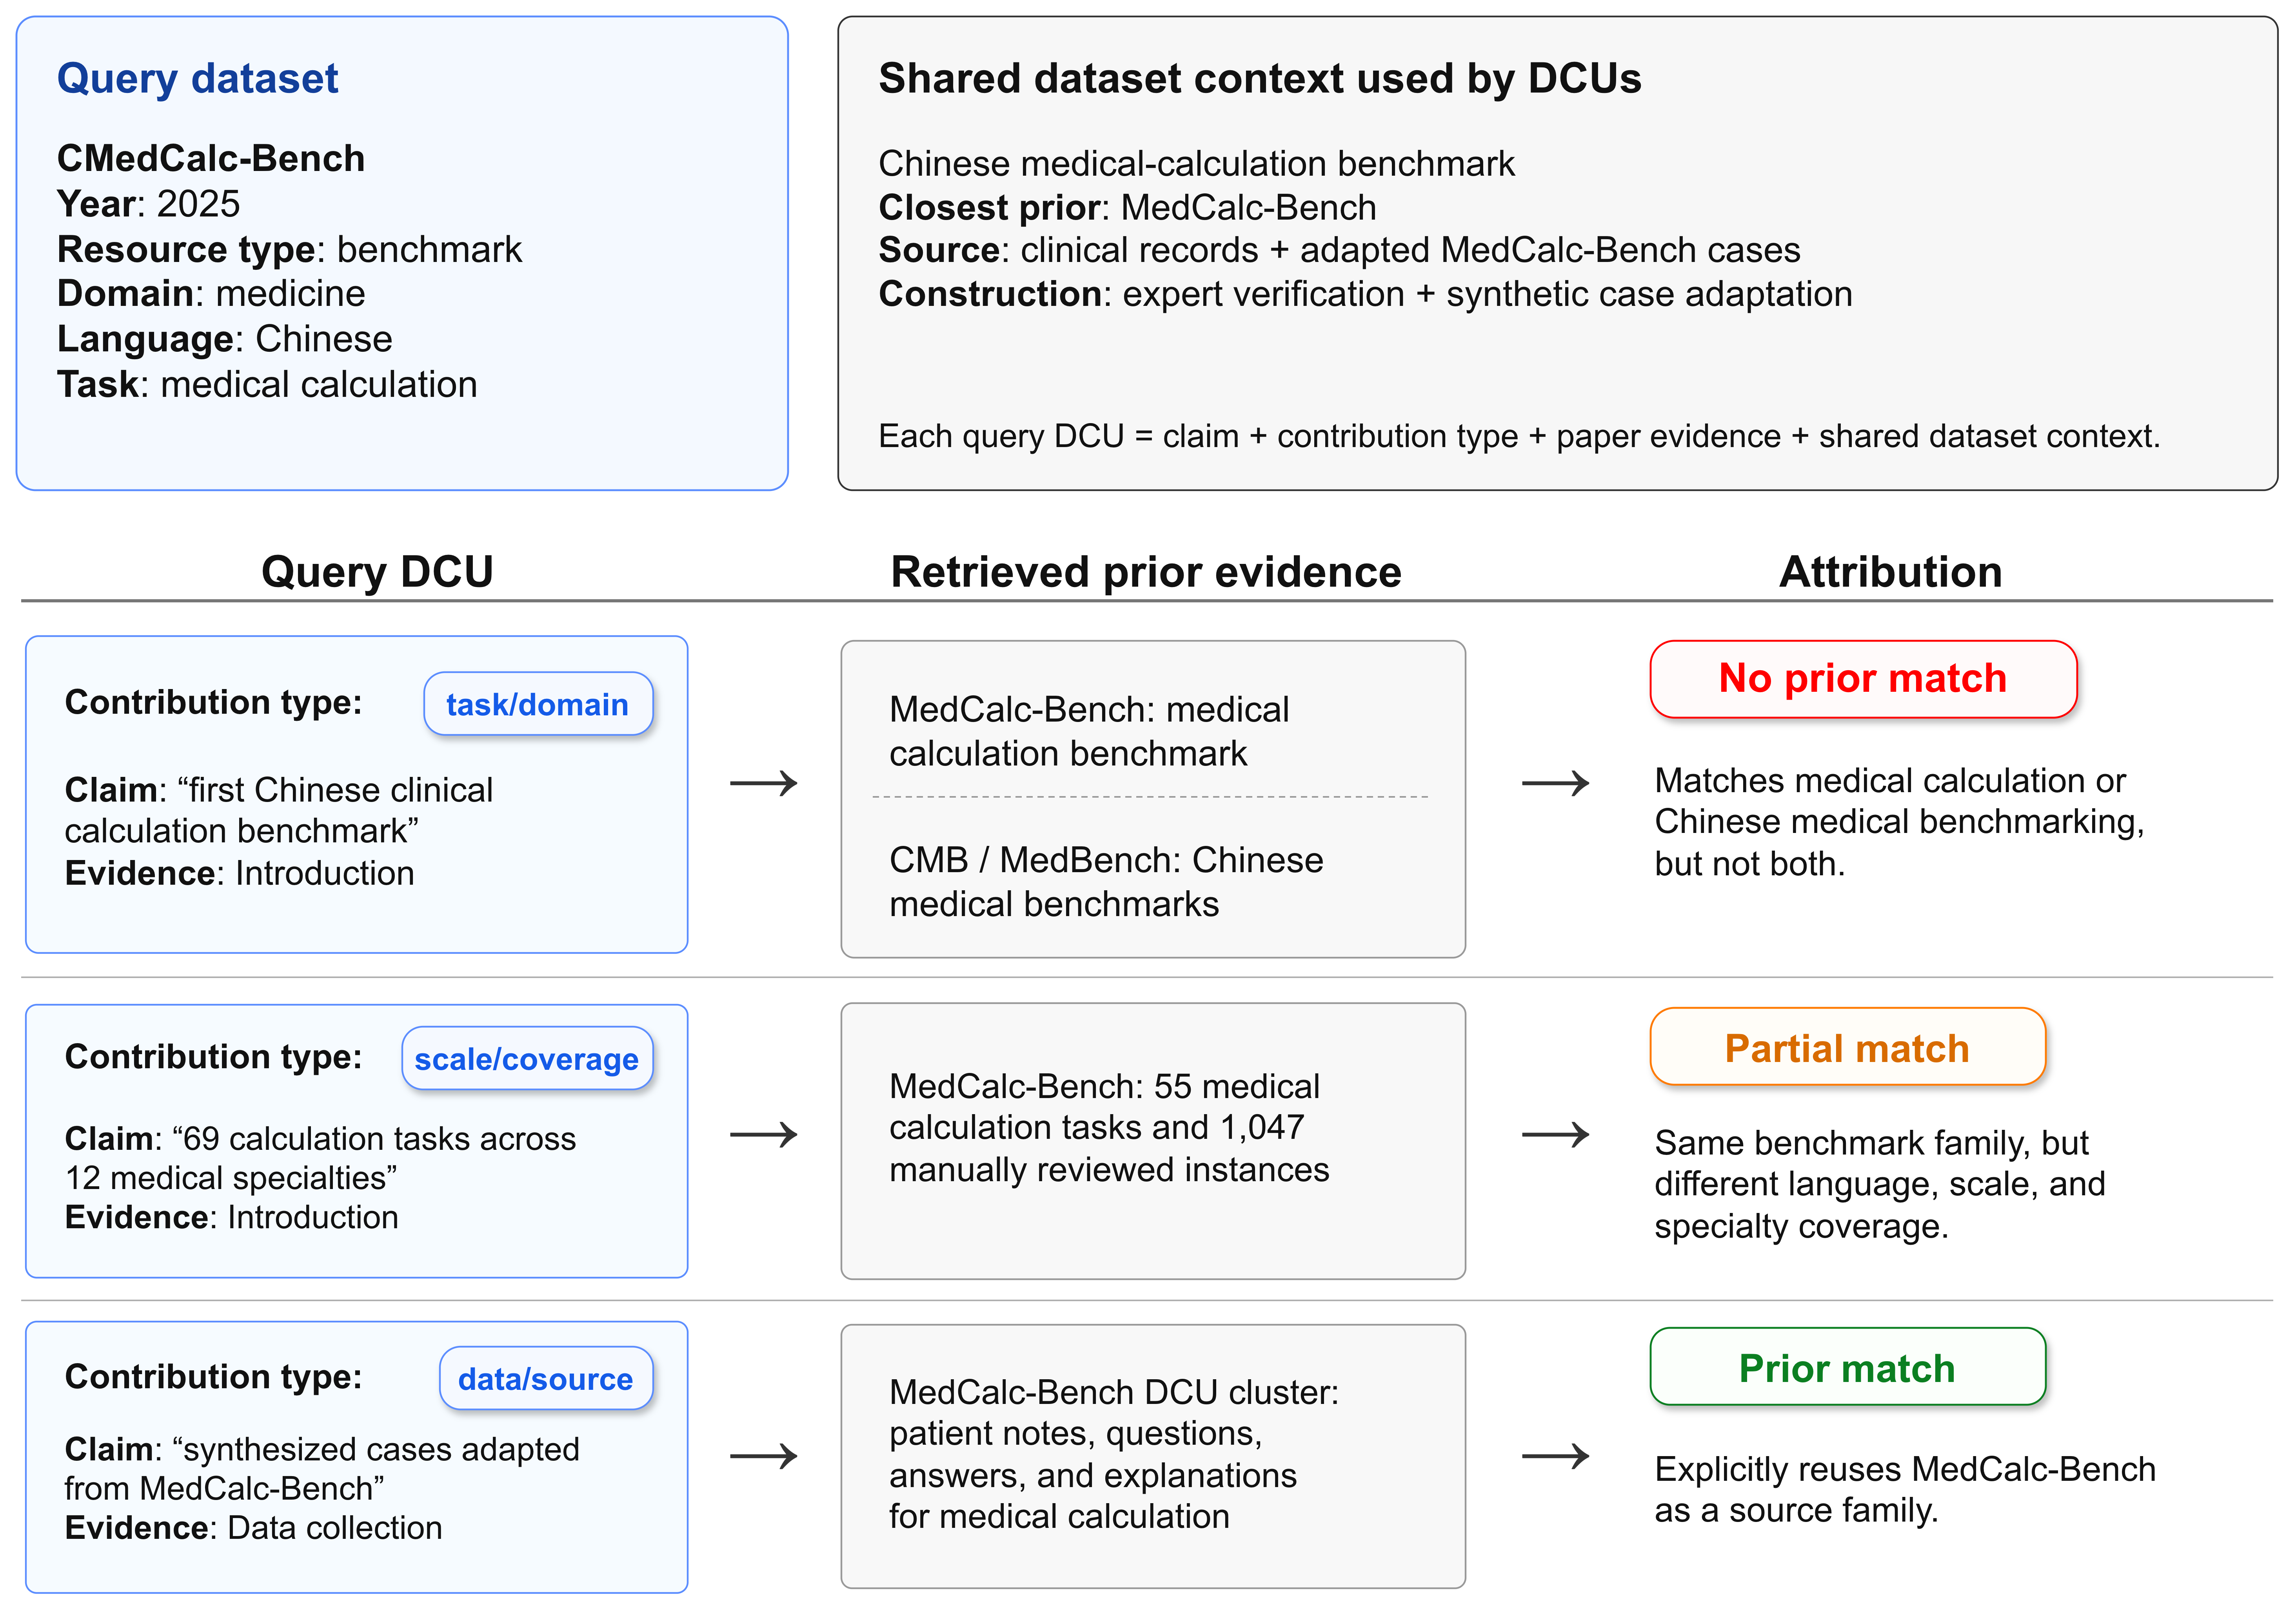
\includegraphics[width=0.70\linewidth]{figures/figure2_cmedcalc_worked_example.png}
\caption{Example of DCU-level prior-evidence attribution for CMedCalc-Bench.}
\label{fig:worked_example}
\end{figure*}

\section{Appendix: Dataset-Paper Classifier Validation}
\label{app:classifier_validation}

The dataset-paper screen is evaluated on a held-out corpus sample annotated by two human reviewers.
Annotators mark whether each paper introduces, substantially modifies, or releases a dataset or benchmark, as opposed to only using existing datasets.
The classifier achieves 0.983--0.993 accuracy against the human labels.
The remaining errors are concentrated in borderline cases: benchmark-analysis papers that include small derived evaluation resources, papers that release prompts or generated outputs rather than a reusable dataset, and papers where a dataset is introduced only in an appendix or project page.
We use this screen as a high-recall entry point for full-text extraction; later stages may still discard records whose extracted dataset entry is invalid or lacks sufficient evidence.

\section{Appendix: Full Retrieval Benchmark Results}
\label{app:full_retrieval_results}

Table~\ref{tab:dcu_retrieval_full} reports the complete retrieval comparison underlying Table~\ref{tab:dcu_retrieval}.
\begin{table*}[h]
\centering
\scriptsize
\setlength{\tabcolsep}{3pt}
\begin{tabular}{lllrrrrr}
\toprule
Family & Representation & Scorer & Hit@1 & Hit@10 & Hit@50 & MRR & nDCG@10 \\
\midrule
\textit{Lower} & Random DCU & Random & 0.000 & 0.037 & 0.175 & 0.016 & 0.010 \\
\midrule
\multicolumn{8}{l}{\textit{Paper-level retrieval: rank papers, then expand paper scores to DCUs}} \\
Paper & Title+abstract & BM25 & 0.281 & 0.669 & 0.831 & 0.403 & 0.441 \\
Paper & Title+abstract & Dense & 0.306 & 0.700 & 0.863 & 0.442 & 0.486 \\
Paper & Title+abstract & Hybrid & 0.306 & 0.713 & 0.900 & 0.445 & 0.482 \\
Paper & Contribution summary & BM25 & 0.294 & 0.681 & 0.838 & 0.424 & 0.457 \\
Paper & Contribution summary & Dense & 0.294 & 0.706 & 0.863 & 0.437 & 0.485 \\
Paper & Contribution summary & Hybrid & 0.319 & 0.756 & 0.900 & 0.465 & 0.508 \\
Paper & Full text & BM25 & 0.269 & 0.606 & 0.787 & 0.378 & 0.414 \\
Paper & Full text & Dense & 0.287 & 0.631 & 0.800 & 0.407 & 0.433 \\
Paper & Full text & Hybrid & 0.325 & 0.681 & 0.863 & 0.446 & 0.482 \\
\midrule
\multicolumn{8}{l}{\textit{Claim-level retrieval without full dataset metadata}} \\
Claim & ACU text & BM25 & 0.188 & 0.431 & 0.619 & 0.263 & 0.226 \\
Claim & ACU text & Dense & 0.225 & 0.412 & 0.669 & 0.289 & 0.230 \\
Claim & ACU text & Hybrid & 0.219 & 0.487 & 0.669 & 0.308 & 0.263 \\
Claim & ACU type+text & BM25 & 0.175 & 0.419 & 0.619 & 0.254 & 0.222 \\
Claim & ACU type+text & Dense & 0.181 & 0.400 & 0.594 & 0.258 & 0.223 \\
Claim & ACU type+text & Hybrid & 0.175 & 0.450 & 0.644 & 0.275 & 0.247 \\
\midrule
\multicolumn{8}{l}{\textit{DCU retrieval: claim text enriched with dataset metadata and paper context}} \\
DCU & Full DCU & BM25 & \textbf{0.456} & 0.812 & 0.956 & 0.586 & 0.597 \\
DCU & Full DCU & Dense & 0.338 & 0.806 & 0.931 & 0.505 & 0.540 \\
DCU & Full DCU & Hybrid & 0.450 & \textbf{0.894} & \textbf{0.963} & \textbf{0.602} & \textbf{0.633} \\
\bottomrule
\end{tabular}
\caption{Full DCU-level prior evidence retrieval results on 160 query DCUs with human-confirmed prior evidence. Bold marks the best result in each column.}
\label{tab:dcu_retrieval_full}
\end{table*}

\section{Appendix: Score Mapping and Relation to Entailment}
\label{app:score_mapping}

The added-information score uses the label mapping in Section~\ref{sec:dataset_profiles}: prior match maps to 0, partial prior match maps to 0.5, and no prior match maps to 1.
This mapping is not intended as a calibrated probability of novelty.
It is an ordinal summary of the evidence relation between a query DCU and retrieved prior DCUs.
The design parallels claim-verification and textual-entailment setups in which evidence may support a claim, contradict it, or fail to provide support \citep{thorne2018fever}.
In our setting, a prior-evidence match means that retrieved prior evidence already expresses the same dataset contribution, so it contributes no added-information mass.
A partial prior-evidence match indicates semantic overlap with an important difference in domain, language, source, annotation protocol, scale, or release setting, so it receives an intermediate score.
A no-prior-match label means that the current evidence index contains no retrieved DCU that matches or partially matches the claim, so it receives the maximum score under the evidence index.
Contradicted and not-comparable labels are rare diagnostics and are excluded from the score rather than forced onto the 0--1 scale.
\section{Appendix: Evidence Adequacy Filtering}
\label{app:evidence_adequacy_details}

For each query DCU, the attribution model produces two adequacy diagnostics in addition to the evidence-match label.
The first diagnostic marks whether the retrieved prior evidence is sufficient to interpret the attribution.
The second flags high missing-prior risk, meaning that the retrieved evidence appears too sparse, too generic, or too mismatched to rule out relevant prior work.
For each dataset record $d$, we aggregate these judgments into three rates:
$r_{\mathrm{insuff}}(d)$, the fraction of DCUs with insufficient retrieved evidence;
$r_{\mathrm{risk}}(d)$, the fraction of DCUs with high missing-prior risk; and
$r_{\mathrm{interp}}(d)$, the fraction of DCUs that remain interpretable for attribution.

We include a dataset record in corpus-level added-information analysis only if:
\begin{equation}
\begin{split}
    &r_{\mathrm{insuff}}(d) \leq 0.50, \\
    &r_{\mathrm{risk}}(d) \leq 0.34, \\
    &r_{\mathrm{interp}}(d) \geq 0.50.
\end{split}
\end{equation}
These thresholds are applied at the dataset-record level.
They are intended as an abstention heuristic: a single high-risk DCU does not exclude a dataset record, but records whose attributions are dominated by sparse or mismatched evidence are excluded from corpus-level score analyses.
All no-prior-match labels are therefore interpreted as no prior match under the retrieved evidence index, not as proof of global novelty.
We do not treat these thresholds as optimized decision boundaries.
They are conservative heuristics chosen before the main corpus-scale analysis to reduce overinterpretation of no-prior-match labels when the retrieved evidence is visibly inadequate.
Because a full threshold-sensitivity analysis is outside the present submission, the main paper avoids claims that depend on exact pass-rate values and instead emphasizes patterns that remain interpretable after filtering.
\section{Appendix: Validation Details}
\label{app:validation_details}
\subsection{Retrieval Benchmark Gold-Label Validation}
\label{app:retrieval_validation_details}
The retrieval benchmark evaluates whether a system can recover specific prior DCUs that humans identify as evidence for a query DCU.
Annotators first inspect cited prior dataset papers and mark which prior DCUs directly or partially match each query DCU.
At evaluation time, the retriever must find those marked prior DCUs from the full prior-DCU evidence index, not merely from the cited papers.
A separate validation audit confirms that 91.3\% of inspected gold prior labels are valid evidence.
Cases with invalid evidence or unresolved annotator disagreement are excluded from the benchmark used in Table~\ref{tab:dcu_retrieval}.

\subsection{Human Audit}
We validate extraction and evidence attribution through human audit.
Because agreement measures depend on annotation design and label distributions, we interpret human agreement as one diagnostic rather than as a complete validity proof \citep{artstein2008intercoder}.
DCU construction is highly reliable: extracted claims are grounded in their evidence spans and assigned the correct contribution type in nearly all audited cases.
For attribution, selected prior evidence is usually relevant, and rationales are grounded in the displayed evidence.
We additionally ask auditors whether they agree with the final evidence-match label given the query DCU, retrieved evidence, selected evidence, and rationale.
Human agreement with final evidence-match labels is reported as an audit of the most subjective step in the pipeline (Table~\ref{tab:human_audit}).
\begin{table}[h]
\centering
\small
\setlength{\tabcolsep}{3pt}
\begin{tabular}{llrr}
\toprule
Component & Metric & N & Value \\
\midrule
DCU & Grounded claim & 276 & 98.6\% \\
DCU & Type accuracy & 276 & 99.3\% \\
Evidence & Precision & 113 & 92.9\% \\
Rationale & Groundedness & 150 & 98.7\% \\
Labels & Human--LLM & 350 & 76.3--77.4\% \\
Labels & Human--human decision & 350 & 92.0\% \\
Labels & Human--human final label & 350 & 90.3\% \\
\bottomrule
\end{tabular}
\caption{Human validation summary. DCU construction, selected evidence, and rationales show strong reliability. Human--LLM agreement reports whether auditors accept the final evidence-match label, chosen from prior match, partial match, no prior match, contradicted, and not comparable, given the displayed query DCU and retrieved evidence.}
\label{tab:human_audit}
\end{table}
Table~\ref{tab:human_audit} separates validation by pipeline component.
The first two rows check whether DCUs are well formed before retrieval: the extracted claim must be supported by its paper evidence span, and the contribution type must be correct.
The evidence and rationale rows check whether the attribution output is grounded in the retrieved prior DCUs.
The label rows evaluate the most judgment-sensitive part of the pipeline, namely whether the final evidence-match label is acceptable given the displayed query DCU and retrieved evidence.
Rejected labels generally reflect boundary disagreements among prior match, partial match, and no prior match, especially when a prior DCU overlaps the query in task or source but differs in domain, scale, annotation protocol, or release setting.
For the 350-case evidence-match label audit, two annotators independently judged whether they accepted the model label and, when rejecting it, supplied a corrected label.
Their binary accept/reject decisions agree in 92.0\% of cases, with Cohen's $\kappa=0.775$.
Their final labels, taking the model label when accepted and the corrected label when rejected, agree in 90.3\% of cases, with Cohen's $\kappa=0.820$.
Both annotators accept the model label in 255 cases, both reject it in 67 cases, and exactly one rejects it in 28 cases.
\subsection{Hosted-Dataset Description Alignment}
Our main DCUs are extracted from author-written dataset papers.
To test whether these paper-derived descriptions are consistent with independently available dataset evidence, we conduct a description-alignment validation on 79 randomly selected datasets with hosted dataset pages.
For each dataset, we collect hosted evidence such as a Hugging Face dataset card, metadata fields, sample rows, GitHub README, or project page.
We then prompt an LLM to write a short dataset description and key claims using only this hosted evidence and explicitly without access to the introducing paper.
We compare this hosted-evidence description against the author-written description and author ACUs; Table~\ref{tab:description_alignment} summarizes the alignment metrics.
\begin{table}[h]
\centering
\small
\begin{tabular}{lrr}
\toprule
Metric & Mean & Median \\
\midrule
Full-description cosine & 0.741 & 0.774 \\
Per-ACU max sim. & 0.557 & 0.575 \\
ACUs with sim. $\geq$ 0.55 & 0.533 & 0.522 \\
ACUs with sim. $<$ 0.35 & 0.133 & 0.059 \\
Synthetic claims aligned & 0.582 & 0.625 \\
\bottomrule
\end{tabular}
\caption{Description-alignment validation on 79 hosted datasets. Synthetic descriptions use hosted dataset evidence without reading the introducing paper.}
\label{tab:description_alignment}
\end{table}
Table~\ref{tab:description_alignment} tests a different question from the human audit.
Instead of asking whether the attribution labels are correct, it checks whether paper-derived dataset descriptions are broadly consistent with independently available hosted evidence.
The full-description cosine compares whole descriptions at the dataset level, while the ACU-level metrics ask whether individual author claims can be recovered from hosted-evidence descriptions.
The synthetic-claims-aligned row checks the reverse direction: whether claims generated from hosted evidence are also reflected in the paper-derived description.
The full-description cosine similarity is high, suggesting that paper descriptions are broadly consistent with hosted dataset documentation.
At the claim level, a majority of author ACUs have high similarity to synthetic descriptions, while only a small fraction fall below the low-alignment threshold.
This validation does not prove that every author claim is correct, but it suggests that paper-derived DCUs are usually grounded in information that can also be recovered from the released dataset documentation.
It also indicates a path for extending our framework to released datasets without accompanying papers.
This study is limited to released datasets with accessible hosted documentation, and similarity-based alignment is not a substitute for factual verification of every claim.
We therefore use it as a consistency check on the source of DCUs, not as evidence that hosted dataset pages can replace papers in the main analysis.
\paragraph{Description-alignment metric definitions.}
We evaluate $N$ introduced datasets ($N{=}79$) with a public Hugging Face or GitHub URL.
For each dataset, we (i) extract author-written text and author ACUs from the introducing paper,
(ii) generate a synthetic description and key claims with an LLM using only hosted-dataset evidence, and
(iii) score alignment with cosine similarity of \texttt{all-MiniLM-L6-v2} embeddings.
Thresholds are set to high similarity $=0.55$ and low similarity $=0.35$.
Table~\ref{tab:description_alignment} reports the mean and median of per-dataset scores; each dataset contributes one value and datasets are weighted equally regardless of how many ACUs they contain.

\begin{itemize}
  \item \textbf{Full-description cosine:} cosine between embeddings of the full author text and the full synthetic text.
  \item \textbf{Per-ACU max similarity:} for each author ACU, the maximum cosine to any synthetic sentence, aggregated within each dataset.
  \item \textbf{ACUs with similarity $\geq 0.55$:} the fraction of author ACUs whose maximum similarity to synthetic text is at least $0.55$.
  \item \textbf{ACUs with similarity $< 0.35$:} the fraction of author ACUs whose maximum similarity to synthetic text is below $0.35$.
  \item \textbf{Synthetic claims aligned:} the fraction of synthetic key claims whose maximum similarity to any author sentence is at least $0.55$.
\end{itemize}
\section{Appendix: Corpus-Scale Diagnostics}
\label{app:corpus_diagnostics}

This appendix reports supporting diagnostics for the corpus-scale findings.
Table~\ref{tab:dcu_type_score_appendix} gives the full contribution-type score decomposition corresponding to Figure~\ref{fig:contribution_directions}.
Table~\ref{tab:construction_score_appendix} reports the full construction-method score table underlying Figure~\ref{fig:llm_score}.
Tables~\ref{tab:relationship_score_appendix} and~\ref{tab:primary_use_score_appendix} report additional descriptive breakdowns by prior-dataset relation and primary use.
Table~\ref{tab:sector_diagnostics_appendix} reports institution-sector diagnostics recovered from the full-text extraction metadata.
These appendix tables are intended as robustness and scope diagnostics rather than additional main-paper findings.
\begin{table*}[h]
\centering
\small
\setlength{\tabcolsep}{4pt}
\begin{tabular}{lrrrr}
\toprule
Contribution type & Records & DCUs & Score mass share & Mean claim score \\
\midrule
Scale/coverage & 8,103 & 9,615 & 30.0\% & 0.687 \\
Annotation/protocol & 6,938 & 8,469 & 19.6\% & 0.512 \\
Task/domain & 5,444 & 6,105 & 17.4\% & 0.557 \\
Data/source & 6,393 & 7,174 & 16.9\% & 0.510 \\
Evaluation/use & 3,256 & 3,682 & 9.6\% & 0.553 \\
Availability/quality & 2,373 & 2,442 & 5.6\% & 0.560 \\
Governance/ethics & 200 & 202 & 0.5\% & 0.569 \\
\bottomrule
\end{tabular}
\caption{Score decomposition by DCU type, excluding the low-frequency \emph{other} category from the main display.}
\label{tab:dcu_type_score_appendix}
\end{table*}
\begin{table*}[h]
\centering
\small
\setlength{\tabcolsep}{4pt}
\begin{tabular}{lrrrr}
\toprule
Construction method & Records & DCUs & Mean score & 95\% CI \\
\midrule
LLM/synthetic & 7,062 & 24,476 & 0.563 & [0.560, 0.566] \\
Human annotated & 1,549 & 5,068 & 0.581 & [0.574, 0.588] \\
Benchmark aggregation & 1,678 & 5,741 & 0.568 & [0.562, 0.575] \\
Translation/multilingual & 613 & 2,175 & 0.564 & [0.554, 0.576] \\
Derived/filtered & 82 & 207 & 0.517 & [0.476, 0.553] \\
Newly collected & 45 & 81 & 0.523 & [0.474, 0.570] \\
\bottomrule
\end{tabular}
\caption{Added-information score by construction method over adequacy-passing 2024--2025 records. Low-frequency categories are retained here as diagnostics but not emphasized in the main figure.}
\label{tab:construction_score_appendix}
\end{table*}
\begin{table*}[h]
\centering
\small
\setlength{\tabcolsep}{4pt}
\begin{tabular}{lrrrr}
\toprule
Prior-dataset relation & Records & DCUs & Mean score & 95\% CI \\
\midrule
Source/reuse & 5,477 & 18,815 & 0.562 & [0.558, 0.565] \\
Comparison/evaluation prior & 5,184 & 18,627 & 0.573 & [0.570, 0.576] \\
No explicit prior mention & 1,156 & 3,215 & 0.553 & [0.547, 0.560] \\
Inspired/shared task & 73 & 248 & 0.552 & [0.525, 0.578] \\
\bottomrule
\end{tabular}
\caption{Prior-dataset relationship diagnostics. Relationship groups are descriptive and may overlap across records; differences in mean score are modest, so this table is used as supporting context rather than a main finding.}
\label{tab:relationship_score_appendix}
\end{table*}
\begin{table*}[h]
\centering
\small
\setlength{\tabcolsep}{4pt}
\begin{tabular}{lrrrr}
\toprule
Primary use & Records & DCUs & Mean score & 95\% CI \\
\midrule
Evaluation/benchmarking & 6,798 & 23,732 & 0.570 & [0.567, 0.573] \\
Training/fine-tuning & 3,709 & 12,168 & 0.556 & [0.552, 0.560] \\
Analysis/research & 515 & 1,796 & 0.580 & [0.568, 0.592] \\
\bottomrule
\end{tabular}
\caption{Added-information score by primary use. Differences are small and are reported as descriptive diagnostics.}
\label{tab:primary_use_score_appendix}
\end{table*}
Table~\ref{tab:sector_diagnostics_appendix} reports an institution-sector diagnostic recovered from the full-text extraction metadata.
Sector differences are small for added-information scores and scale/coverage profiles, but larger for LLM-assisted construction and release practices.
\begin{table*}[h]
\centering
\small
\setlength{\tabcolsep}{4pt}
\begin{tabular}{lrrrrrr}
\toprule
Sector & Records & Mean score & LLM share & Scale score mass & Released & Open access \\
\midrule
Academic only & 6,600 & 0.568 & 60.4\% & 30.3\% & 72.0\% & 73.5\% \\
Academic--industry & 3,430 & 0.562 & 68.0\% & 30.0\% & 73.2\% & 74.9\% \\
Industry only & 787 & 0.565 & 74.1\% & 29.2\% & 55.9\% & 57.9\% \\
\bottomrule
\end{tabular}
\caption{
Institution-sector diagnostics over adequacy-passing records.
Scores are evidence-conditioned added-information scores.
Scale score mass is the share of total sector score mass contributed by scale/coverage DCUs.
}
\label{tab:sector_diagnostics_appendix}
\end{table*}
\end{document}
